\documentclass[conference]{IEEEtran}
\IEEEoverridecommandlockouts
\usepackage{cite}
\usepackage{amsmath,amssymb}
\usepackage{graphicx}
\usepackage{xcolor}
\usepackage{textcomp}
\usepackage{booktabs}
\usepackage{array}
\usepackage{multirow}
\usepackage{listings}
\usepackage{tikz}
\usetikzlibrary{positioning,arrows.meta,shapes.geometric}
\usepackage[hidelinks]{hyperref}
\usepackage{url}
\renewcommand{\ttdefault}{cmtt}

\definecolor{kw}{RGB}{124,58,237}
\definecolor{cm}{RGB}{120,128,140}
\lstdefinelanguage{MetroLang}{
  morekeywords={board,ride,to,change,exit},
  sensitive=false,
  morecomment=[l]{//},
  morecomment=[l]{\#},
  morestring=[b]"
}
\lstset{
  basicstyle=\ttfamily\footnotesize,
  keywordstyle=\color{kw},
  commentstyle=\color{cm}\itshape,
  columns=fullflexible,
  keepspaces=true,
  frame=single,
  framesep=3pt,
  xleftmargin=4pt,
  xrightmargin=4pt,
  aboveskip=6pt,
  belowskip=6pt,
  breaklines=true
}

\begin{document}

\title{MetroLang: A Domain-Specific Compiler for Delhi Metro Journeys with Phase-by-Phase Interactive Visualization}

\author{
\IEEEauthorblockN{Raman Luhach, Ritesh Patil, Rachit Kumar, Meghavi Rao, Harshal Nerpagar}
\IEEEauthorblockA{\textit{Team Semester Survivors} (Team Lead: Raman Luhach) --- Compiler Design Project\\
\textit{AI Product Engineering Track}}
}

\maketitle

\begin{abstract}
This paper presents \emph{MetroLang}, a small domain-specific language for describing journeys on the Delhi Metro, together with a complete compiler for it. A program such as \texttt{board Rajiv Chowk; ride Yellow to Hauz Khas; change Magenta; ride to Botanical Garden; exit} passes through all six classical compiler phases: lexical analysis, syntax analysis, semantic analysis, intermediate code generation, optimization and code generation. The output is a journey card with stops, interchanges, an estimated time and fare, and an animated train on a schematic metro map. The compiler is checked against real network data: six lines, 203 stations and 17 interchanges, taken from public line articles. It enforces 15 semantic rules, such as allowing line changes only at real interchanges, and reports lexical, syntactic and semantic errors with line and column information, recovery, and ``did you mean'' suggestions. Four peephole optimizations run to a fixed point over a quadruple-based intermediate representation, and a Dijkstra-based advisor suggests faster routes. Every intermediate state (tokens, parse tree, AST, symbol table, IR, optimized IR and target code) is shown in an interactive browser application. An automated suite of 81 tests verifies correctness. The system was built on the AI Product Engineering track using a generative-AI coding agent, with every phase checked by tests and visual inspection.
\end{abstract}

\begin{IEEEkeywords}
compiler design, domain-specific language, lexical analysis, recursive-descent parsing, semantic analysis, intermediate representation, peephole optimization, visualization, Delhi Metro
\end{IEEEkeywords}

%=====================================================================
\section{Introduction}
Compiler courses usually present the phases of a compiler in the context of general-purpose languages, where intermediate results such as token streams, parse trees and three-address code are hard to see and harder to relate to everyday experience. A domain-specific language (DSL) with a familiar real-world meaning makes each phase concrete: a token is a word of a journey, a semantic error is a journey that is physically impossible, and an optimization is a shorter trip.

We chose the \emph{Delhi Metro Journey} use case because it has a simple, regular syntax but rich, real semantics. Whether a program is valid depends on facts about a real network: which stations lie on which line, where lines intersect, and how branches split. These facts naturally become a \emph{symbol table}, and the passenger's position becomes the state carried through semantic analysis.

The main contributions of this work are:
\begin{itemize}
\item the design of MetroLang, a small LL(1) language with five statement forms (Section~\ref{sec:lang});
\item a complete six-phase compiler with error recovery in the parser and 15 semantic rules plus 4 warnings checked against real data (Sections~\ref{sec:method}--\ref{sec:impl});
\item a quadruple IR with four peephole optimizations and a graph-based route advisor (Section~\ref{sec:opt});
\item an interactive web application that shows the output of every phase and animates the generated journey (Section~\ref{sec:ui});
\item an automated test suite of 81 tests and an evaluation of correctness and performance (Section~\ref{sec:results}).
\end{itemize}

%=====================================================================
\section{Background}
The classical compiler pipeline~\cite{aho2006} separates \emph{analysis} (lexical, syntax and semantic) from \emph{synthesis} (intermediate code, optimization and code generation), with a symbol table shared by all phases. Lexical analysers are specified with regular expressions, and syntax with context-free grammars. Grammars in which one token of lookahead decides every production (LL(1)) can be parsed by hand-written recursive-descent parsers~\cite{appel1998,cooper2011}. Peephole optimization, introduced by McKeeman~\cite{mckeeman1965}, improves code by rewriting short windows of adjacent instructions. Classic educational DSLs such as Logo show that a small language with immediate visual output is an effective way to teach programming concepts~\cite{papert1980}. Our route advisor uses Dijkstra's shortest-path algorithm~\cite{dijkstra1959}, and our error suggestions use Levenshtein edit distance~\cite{levenshtein1966}.

%=====================================================================
\section{Language Design}\label{sec:lang}

\subsection{Statements}
A MetroLang program is a sequence of statements terminated by semicolons. The final semicolon is optional, matching the example in the project brief:
\begin{lstlisting}[language=MetroLang]
board Rajiv Chowk;          // start
ride Yellow to Hauz Khas;   // ride a line
change Magenta;             // change at interchange
ride to Botanical Garden;   // continue on line
exit
\end{lstlisting}
Station names may be written plainly or in quotes, and matching ignores case and punctuation, so \texttt{Dilli Haat INA}, \texttt{"Dilli Haat - INA"} and the alias \texttt{INA} all refer to the same station. Comments use \texttt{//}, \texttt{\#} or \texttt{/*\,\ldots\,*/}.

\subsection{Lexical Specification}
Table~\ref{tab:tokens} lists the token classes. Keywords and the six line names are recognised case-insensitively. Station names are sequences of \texttt{WORD}, \texttt{NUMBER}, \texttt{HYPHEN}, \texttt{COMMA} and \texttt{PAREN} tokens, which supports names such as \emph{Rohini Sector 18, 19} and \emph{Shaheed Sthal (New Bus Adda)}.

\begin{table}[t]
\caption{Token classes of MetroLang}\label{tab:tokens}
\centering\footnotesize
\begin{tabular}{@{}l l l@{}}
\toprule
\textbf{Token} & \textbf{Pattern} & \textbf{Example}\\
\midrule
KEYWORD & \texttt{board|ride|to|change|exit} & \texttt{ride}\\
LINE & \texttt{yellow|blue|violet|magenta|red|pink} & \texttt{Yellow}\\
WORD & \texttt{[A-Za-z][A-Za-z0-9.'-]*} & \texttt{Vihar-I}\\
NUMBER & \texttt{[0-9]+} & \texttt{21}\\
STRING & \texttt{"[\^{}"\textbackslash n]*"} & \texttt{"INA"}\\
SEMICOLON & \texttt{;} & \texttt{;}\\
COMMENT & \texttt{//.*\,|\,\#.*\,|\,/*\ldots*/} & \texttt{// hi}\\
\bottomrule
\end{tabular}
\end{table}

\subsection{Grammar}
The syntax is given by the following context-free grammar:
\begin{lstlisting}
<program> ::= <stmt>* EOF
<stmt>    ::= <board> | <ride> | <change> | <exit>
<board>   ::= "board" <station> ";"
<ride>    ::= "ride" [ LINE ] "to" <station> ";"
<change>  ::= "change" LINE ";"
<exit>    ::= "exit" ";"
<station> ::= STRING | <part> { <part> }
<part>    ::= WORD | NUMBER | HYPHEN | COMMA | PAREN
\end{lstlisting}
Because the FIRST sets of the four statement forms are disjoint (\{\texttt{board}\}, \{\texttt{ride}\}, \{\texttt{change}\}, \{\texttt{exit}\}), the grammar is LL(1).

%=====================================================================
\section{Methodology and Architecture}\label{sec:method}

\subsection{Pipeline}
Fig.~\ref{fig:pipeline} shows the architecture. Each phase is a separate module with a clear input and output, and a driver runs the phases in order. A phase runs only if the earlier phases succeeded, except that the parser still runs after lexical errors so that more errors can be reported in one compilation. The metro network is loaded once and serves as the pre-populated symbol table.

\begin{figure}[t]
\centering
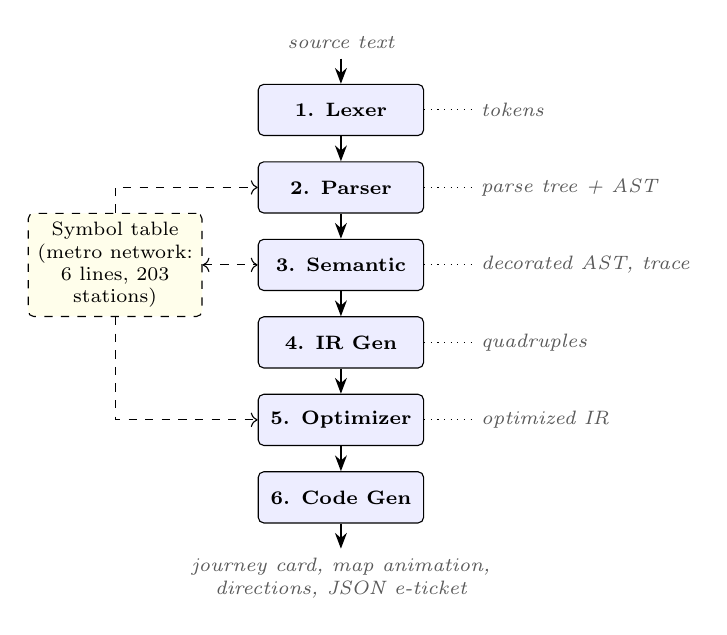
\begin{tikzpicture}[
  node distance=3.2mm and 2.4mm,
  ph/.style={draw, rounded corners=2pt, fill=blue!7, minimum width=21mm, minimum height=6.5mm, font=\scriptsize\bfseries, align=center},
  io/.style={font=\scriptsize\itshape, text=black!65, align=center},
  ar/.style={-{Stealth[length=2mm]}, thick}]
\node[io] (src) {source text};
\node[ph, below=of src] (lex) {1. Lexer};
\node[ph, below=of lex] (par) {2. Parser};
\node[ph, below=of par] (sem) {3. Semantic};
\node[ph, below=of sem] (ir) {4. IR Gen};
\node[ph, below=of ir] (opt) {5. Optimizer};
\node[ph, below=of opt] (gen) {6. Code Gen};
\node[io, below=of gen] (out) {journey card, map animation,\\ directions, JSON e-ticket};
\node[io, right=6mm of lex] (t1) {tokens};
\node[io, right=6mm of par] (t2) {parse tree + AST};
\node[io, right=6mm of sem] (t3) {decorated AST, trace};
\node[io, right=6mm of ir] (t4) {quadruples};
\node[io, right=6mm of opt] (t5) {optimized IR};
\node[draw, dashed, rounded corners=2pt, font=\scriptsize, align=center, left=7mm of sem, fill=yellow!8] (sym) {Symbol table\\(metro network:\\6 lines, 203\\stations)};
\draw[ar] (src)--(lex); \draw[ar] (lex)--(par); \draw[ar] (par)--(sem);
\draw[ar] (sem)--(ir); \draw[ar] (ir)--(opt); \draw[ar] (opt)--(gen); \draw[ar] (gen)--(out);
\foreach \a/\b in {lex/t1,par/t2,sem/t3,ir/t4,opt/t5} \draw[-, dotted] (\a)--(\b);
\draw[<->, dashed] (sym.east)--(sem.west);
\draw[->, dashed] (sym.north) |- (par.west);
\draw[->, dashed] (sym.south) |- (opt.west);
\end{tikzpicture}
\caption{MetroLang compiler architecture. Every intermediate result (right) is shown in the user interface.}
\label{fig:pipeline}
\end{figure}

\subsection{Network Data}
Station sequences and interchanges for the Yellow, Blue (main line and Vaishali branch), Violet, Magenta, Red and Pink lines were taken from the Wikipedia article for each line~\cite{wiki-yellow,wiki-blue,wiki-violet,wiki-magenta,wiki-red,wiki-pink}, and checked by automated integrity tests (Section~\ref{sec:results}). Each line is stored as one or more ordered \emph{routes}, which models the Blue Line split at Yamuna Bank. Interchanges are derived automatically as stations that lie on two or more lines, giving 17 interchanges, including Kashmere Gate with three lines. Approximate coordinates are stored only for drawing the map; missing positions are interpolated along each line.

\subsection{Development Methodology}
Following the AI Product Engineering track, the application was built iteratively with a generative-AI coding agent. The team defined the requirements and rubric mapping. The agent proposed the language design, collected the network data, and implemented the phases one at a time. After each phase, automated tests and smoke runs checked behaviour, and screenshots of the interface rendered in a headless browser were inspected to find visual defects. Section~\ref{sec:ai} lists the defects found and fixed during this process.

%=====================================================================
\section{Implementation}\label{sec:impl}
The compiler is written in plain JavaScript (about 1{,}100 lines for the compiler and 1{,}200 for the interface), with no external dependencies. It runs in any modern browser, and also under Node.js for testing.

\subsection{Lexical Analysis}
The scanner reads the input from left to right and, at each position, tries patterns in a fixed order: whitespace, comments, punctuation, quoted strings, numbers and words. A matched word is then classified as a \texttt{KEYWORD}, a \texttt{LINE} or a plain \texttt{WORD}. Every token records its type, lexeme, line, column and length. The same tokens drive the syntax highlighting in the editor, so what the user sees matches exactly how the lexer tokenised the code. Lexical errors are an illegal character (L01), an unterminated string (L02), an unterminated block comment (L03) and an empty string (L04). After an error the scanner skips the offending character and continues.

\subsection{Syntax Analysis}
A recursive-descent parser has one function per non-terminal and builds two trees at the same time: a concrete \emph{parse tree}, which contains every grammar rule and terminal, and an \emph{abstract syntax tree}, whose nodes are \texttt{Board}, \texttt{Ride}, \texttt{Change} and \texttt{Exit} with their station and line children. Two recovery strategies are used:
\begin{itemize}
\item \emph{Phrase-level recovery}: a missing \texttt{;} or \texttt{to} is reported and then assumed to be present.
\item \emph{Panic-mode recovery}: on any other error, tokens are skipped up to the next \texttt{;} or statement keyword.
\end{itemize}
This lets a single compilation report, for example, an unknown statement \texttt{bord} (with the suggestion \emph{board}), an unknown line \texttt{Yelow} (\emph{Yellow}) and a \texttt{change} without a line, all at once.

\subsection{Semantic Analysis and Symbol Table}
The analyser walks the AST while keeping the passenger state $\langle$\emph{boarded, exited, station, line}$\rangle$. Every station and line name is resolved through the symbol table, and the resolved entry (official name, type, lines served, references) decorates the AST. Table~\ref{tab:rules} lists the rules. For an unknown name, the analyser ranks all known names by Levenshtein distance and suggests the closest. To avoid cascading errors, once a statement fails the analyser stops checking position-dependent rules but still checks name resolution and journey structure. A per-statement trace of the passenger state is recorded and shown in the interface.

\begin{table}[t]
\caption{Semantic rules (errors S01--S15, warnings W01--W04)}\label{tab:rules}
\centering\footnotesize
\begin{tabular}{@{}l p{6.6cm}@{}}
\toprule
\textbf{Code} & \textbf{Rule}\\
\midrule
S01 & The station must exist (with an edit-distance suggestion)\\
S02 / S03 & The journey starts with \texttt{board}; board only once\\
S04 & The first \texttt{ride} must name a line\\
S05 / S06 & The boarding and destination stations must be on the line\\
S07 & \texttt{change} is allowed only at an interchange\\
S08 & The new line must stop at that interchange\\
S09 / S10 & No change to the current line; no ride to the current station\\
S11 / S12 & The journey ends with \texttt{exit}; nothing after \texttt{exit}\\
S13 & Both stations must be on the same branch (Blue Line split)\\
S14 & Riding a different line requires \texttt{change}\\
S15 & \texttt{change} requires a line already being ridden\\
\midrule
W01--W04 & Loop, consecutive changes, board-and-exit only, change just before exit\\
\bottomrule
\end{tabular}
\end{table}

\subsection{Intermediate Code Generation}
The checked journey is translated into quadruples $(\mathit{op}, \mathit{arg}_1, \mathit{arg}_2, \mathit{result})$, as shown in Table~\ref{tab:ir}. Generating the IR also computes what the source leaves implicit: the direction of travel (the terminus the train runs towards), the number of stops, the list of stations in between, and the distance and time of each segment.

\begin{table}[t]
\caption{IR for the brief's example program}\label{tab:ir}
\centering\footnotesize
\begin{tabular}{@{}c l l l l@{}}
\toprule
\# & \textbf{op} & \textbf{arg1} & \textbf{arg2} & \textbf{result}\\
\midrule
1 & BOARD & Rajiv Chowk & -- & --\\
2 & RIDE & Yellow & Rajiv Chowk & Hauz Khas \hfill(9 stops)\\
3 & CHANGE & Yellow & Magenta & Hauz Khas\\
4 & RIDE & Magenta & Hauz Khas & Botanical Garden \hfill(13)\\
5 & EXIT & Botanical Garden & -- & --\\
\bottomrule
\end{tabular}
\end{table}

\subsection{Optimization}\label{sec:opt}
The optimizer applies peephole rewrites to adjacent IR instructions and repeats until no rule applies (a fixed point). Each rewrite keeps the starting and ending station unchanged:
\begin{itemize}
\item \textbf{O1 Merge rides}: $\mathrm{RIDE}\,L\,A{\to}B;\ \mathrm{RIDE}\,L\,B{\to}C \Rightarrow \mathrm{RIDE}\,L\,A{\to}C$ when the direction is the same.
\item \textbf{O2 Remove detour}: the same pattern with a reversal of direction collapses to $A{\to}C$. If $C{=}A$, both rides are deleted.
\item \textbf{O3 Merge changes}: $\mathrm{CHANGE}\,x{\to}y;\ \mathrm{CHANGE}\,y{\to}z \Rightarrow \mathrm{CHANGE}\,x{\to}z$. Both are deleted if $x{=}z$.
\item \textbf{O4 Dead change}: $\mathrm{CHANGE};\ \mathrm{EXIT} \Rightarrow \mathrm{EXIT}$.
\item \textbf{O5 Route advisor}: Dijkstra's algorithm over (station, line) states, with hop times as edge weights and a 5-minute penalty per line change, finds the fastest route. If it is clearly faster, it is offered as advice and as generated MetroLang code. The user's route is not changed.
\end{itemize}
A rewrite is applied only if the merged ride is possible on a single train. For example, Noida Sector 18$\to$Yamuna Bank$\to$Vaishali is never merged, because no single Blue Line train serves both branches.

\subsection{Code Generation}
The optimized IR is translated into four targets: (i) a journey summary used by the journey card, (ii) an animation path of station coordinates and line colours, (iii) plain-English directions, and (iv) a machine-readable JSON e-ticket. In addition, an optimized MetroLang program is regenerated from the optimized IR. The estimated time is
\begin{equation}
T = \sum_{\text{rides}} n_i\,\frac{d_i}{v}\cdot 60 \;+\; 5\,c \;+\; 3 \ \text{minutes},
\end{equation}
where $n_i$ is the number of stops on ride $i$, $d_i$ the average inter-station distance of that line, $v=36$\,km/h, and $c$ the number of changes. The fare follows the DMRC distance slabs (Rs.~11, 21, 32, 43, 54 and 64). Both values are shown as estimates.

\subsection{Interactive User Interface}\label{sec:ui}
The browser application has a syntax-highlighted editor (with line numbers, error squiggles and live compilation as the user types), a six-stage pipeline bar that shows the status and run time of each phase, and ten tabs: Tokens, Parse Tree, AST, Symbol Table, Semantic, IR, Optimizer, Output, Target Code and Network. Parse trees and ASTs are drawn as SVG trees that can be panned and zoomed, and clicking a node highlights its source. The Output tab draws all six lines on a schematic map with the Yamuna river for orientation, highlights the compiled route, and animates a train that pauses at interchanges while a timeline in the journey card follows its progress (Fig.~\ref{fig:output}). An optional cinematic 3D view, built with Three.js~\cite{threejs}, lifts the same coordinates into a scene with elevated glowing tubes for the lines, platforms on pillars, and a three-coach train. A camera director switches between a fly-in, a chase camera, side tracking shots, an orbit around each interchange during a line change, and a final pull-back over the whole route. A step mode walks through the phases one at a time, and 24 built-in examples cover valid journeys, optimizations and every error class.

\begin{figure*}[t]
\centering
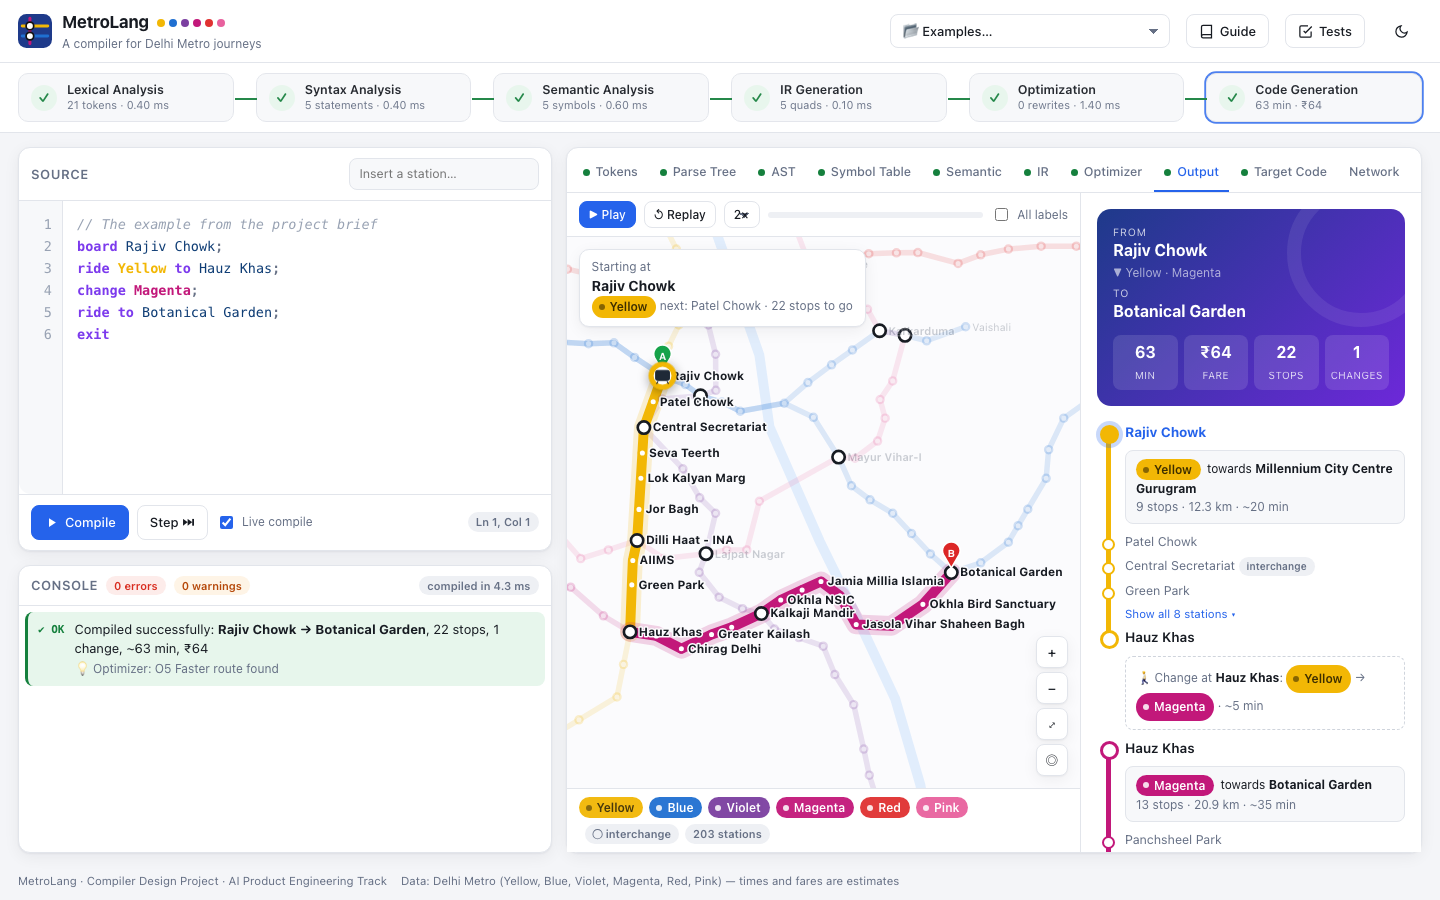
\includegraphics[width=0.92\textwidth]{figures/output-journey.png}
\caption{Output tab: pipeline status, editor, console, animated route on the metro map, and the generated journey card.}
\label{fig:output}
\end{figure*}

\begin{figure}[t]
\centering
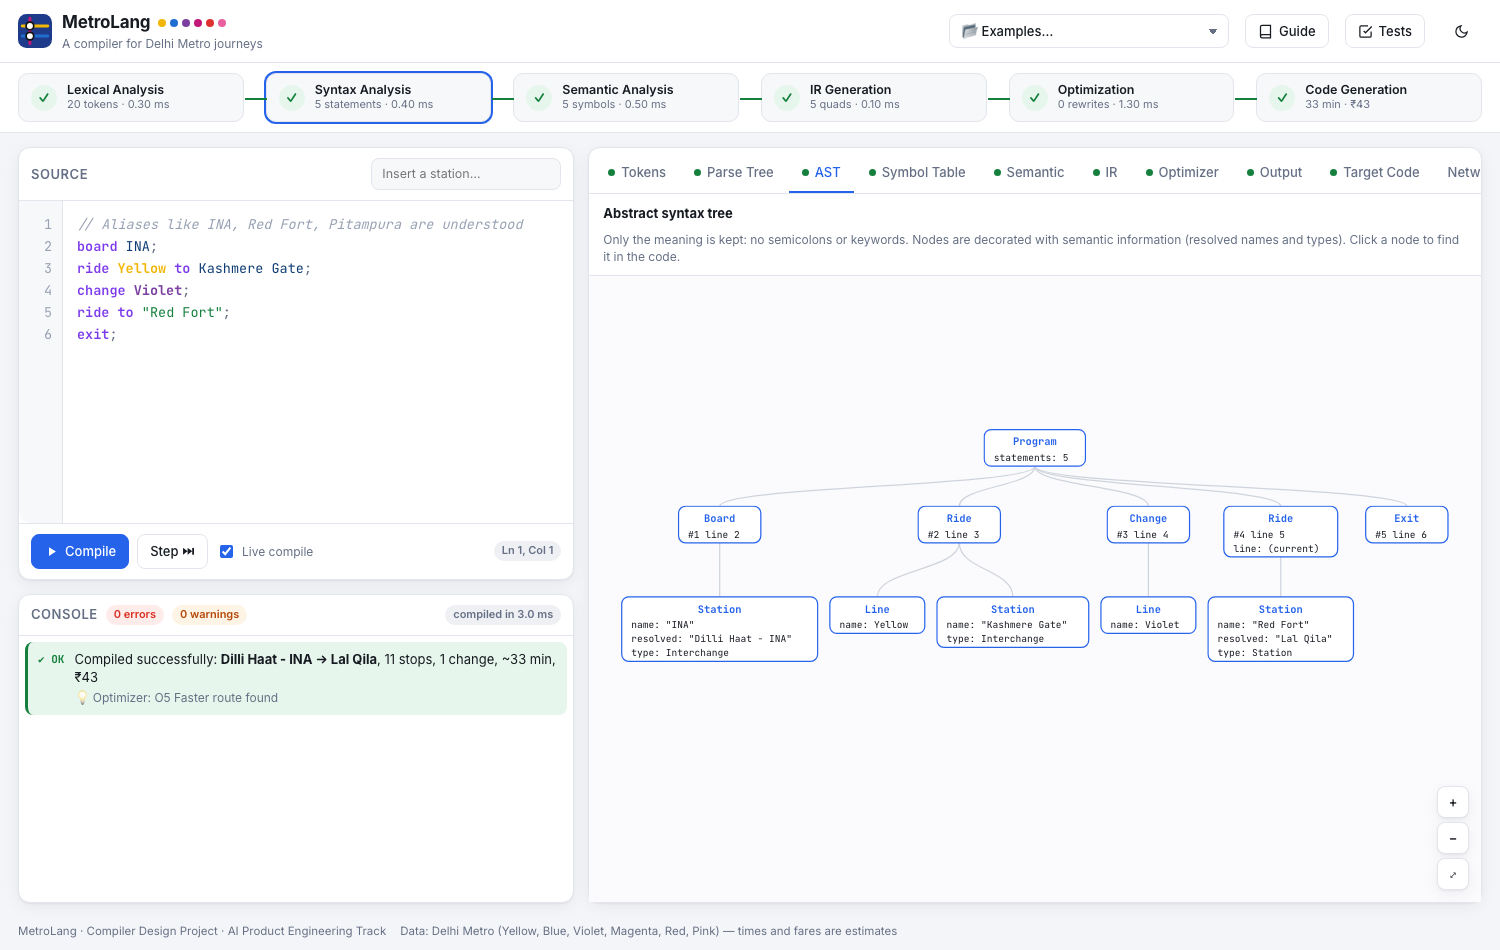
\includegraphics[width=\columnwidth]{figures/ast.png}
\caption{AST decorated with semantic information: aliases resolved (INA $\to$ Dilli Haat - INA, Red Fort $\to$ Lal Qila) and station types.}
\label{fig:ast}
\end{figure}

%=====================================================================
\section{Error Handling}
Table~\ref{tab:errors} summarises the error classes. Each diagnostic carries a code, a message, a line and column, a length (used for the red underline) and a hint. Clicking a diagnostic moves the editor cursor to its location. A phase with errors turns red in the pipeline, and the phases after it are marked as skipped. Fig.~\ref{fig:sem} shows a semantic error at a station that is not an interchange, along with the rule checklist.

\begin{table}[t]
\caption{Error classes and examples}\label{tab:errors}
\centering\footnotesize
\begin{tabular}{@{}l l p{4.4cm}@{}}
\toprule
\textbf{Phase} & \textbf{Codes} & \textbf{Example diagnostics}\\
\midrule
Lexical & L01--L04 & Illegal character ``@''; unterminated string\\
Syntax & P01--P10 & Missing ``;''; missing ``to''; unknown line ``Yelow'' --- did you mean Yellow?\\
Semantic & S01--S15 & Unknown station ``Rajiv Chok'' --- did you mean Rajiv Chowk?; Green Park is not an interchange; no direct Blue Line train to Vaishali\\
Warning & W01--W04 & Journey loops back to a station\\
\bottomrule
\end{tabular}
\end{table}

\begin{figure}[t]
\centering
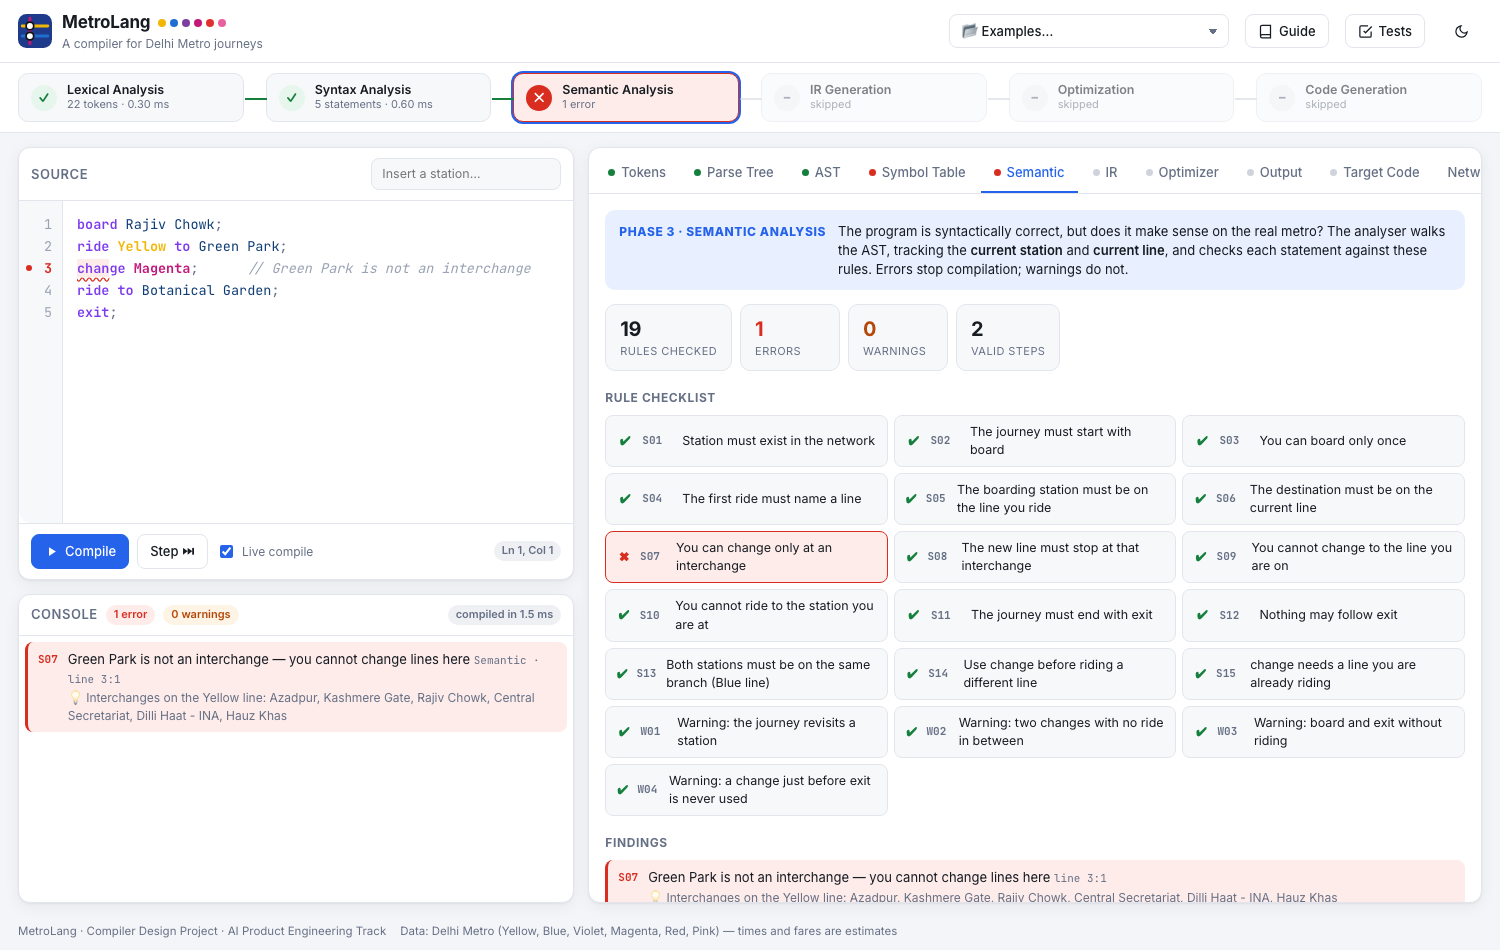
\includegraphics[width=\columnwidth]{figures/semantic-errors.png}
\caption{A semantic error (S07): changing lines at Green Park. The hint lists the valid interchanges on the Yellow Line.}
\label{fig:sem}
\end{figure}

%=====================================================================
\section{Results and Evaluation}\label{sec:results}

\subsection{Test Suite}
The suite runs both from the command line (\texttt{node tests/run-tests.js}) and inside the application. All 81 tests pass (Table~\ref{tab:tests}). The compiler tests check exact stop counts and directions against the published station order (for example, Rajiv Chowk to Hauz Khas is 9 stops on the Yellow Line, and from Hauz Khas towards Kashmere Gate the direction is \emph{towards Samaypur Badli}), every lexical, syntax and semantic error code, every warning, and every optimization rule.

\begin{table}[t]
\caption{Automated test results}\label{tab:tests}
\centering\footnotesize
\begin{tabular}{@{}l r r@{}}
\toprule
\textbf{Category} & \textbf{Tests} & \textbf{Passed}\\
\midrule
Data integrity (lines, interchanges, aliases, connectivity) & 8 & 8\\
Valid programs (stops, direction, fare, aliases) & 10 & 10\\
Lexical errors & 3 & 3\\
Syntax errors (incl.\ multiple errors per run) & 9 & 9\\
Semantic errors (S01--S15, no cascades) & 16 & 16\\
Warnings (W01--W04) & 4 & 4\\
Optimizations (O1--O5, start/end preserved) & 7 & 7\\
Example programs & 24 & 24\\
\midrule
\textbf{Total} & \textbf{81} & \textbf{81}\\
\bottomrule
\end{tabular}
\end{table}

\subsection{Sample Compilations}
Table~\ref{tab:samples} shows results for representative programs. The optimizer demo program shrinks from 11 to 5 IR instructions (and from 51 to 31 estimated minutes) by applying O1, O2, O3 and O4 in sequence (Fig.~\ref{fig:opt}). For the brief's own example, the route advisor points out that the Blue Line runs directly from Rajiv Chowk to Botanical Garden.

\begin{table}[t]
\caption{Sample compilations (time and fare are estimates)}\label{tab:samples}
\centering\footnotesize
\setlength{\tabcolsep}{3.2pt}
\begin{tabular}{@{}l r r r r l@{}}
\toprule
\textbf{Program} & \textbf{Stops} & \textbf{Chg.} & \textbf{Min} & \textbf{Rs.} & \textbf{IR (opt.)}\\
\midrule
Brief example & 22 & 1 & 63 & 64 & 5$\to$5 (O5)\\
Kashmere Gate$\to$T1 Airport & 19 & 1 & 54 & 54 & 5$\to$5\\
Dwarka$\to$Shaheed Sthal (4 lines) & 63 & 3 & 154 & 64 & 9$\to$9 (O5)\\
Noida City Ctr.$\to$Vaishali & 17 & 0 & 36 & 43 & 4$\to$4\\
Faridabad$\to$Rithala & 46 & 1 & 112 & 64 & 5$\to$5\\
Optimizer demo & 10 & 1 & 31 & 43 & 11$\to$5 (O1--O4)\\
\bottomrule
\end{tabular}
\end{table}

\begin{figure}[t]
\centering
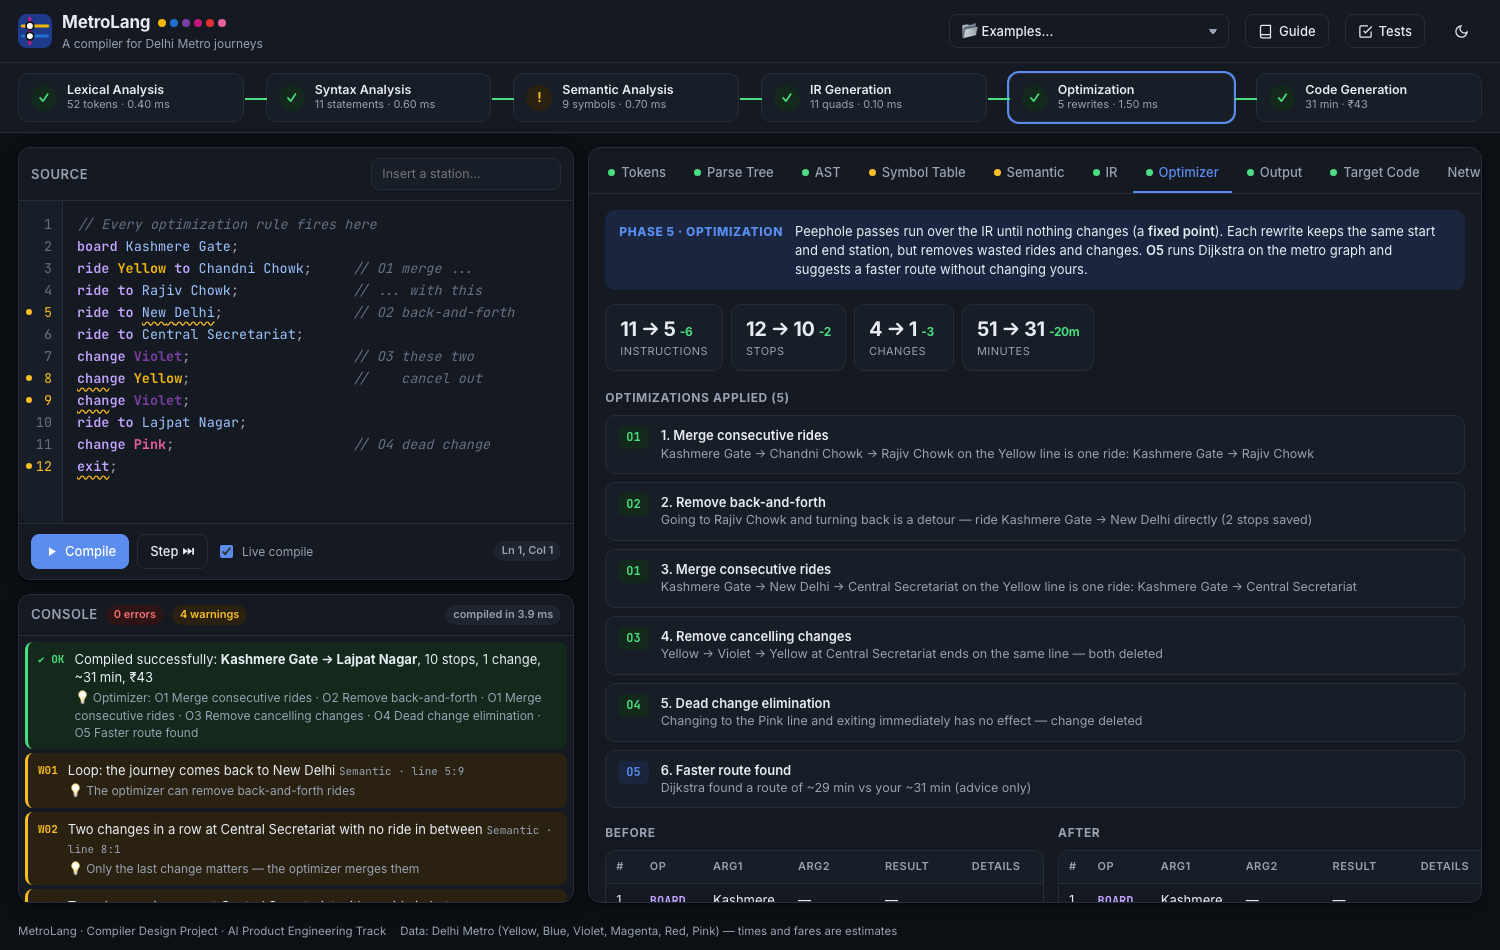
\includegraphics[width=\columnwidth]{figures/optimizer.png}
\caption{Optimizer tab: the applied rewrites, the cost reduction (11$\to$5 instructions, 51$\to$31 minutes) and the before/after IR.}
\label{fig:opt}
\end{figure}

\subsection{Performance}
Measured over 50 runs per program under Node.js, a full six-phase compilation of each example takes between 0.01\,ms and 1.5\,ms. The slowest cases are programs that run the Dijkstra advisor or the edit-distance search over all station names. This is fast enough to recompile on every keystroke.

%=====================================================================
%=====================================================================
\section{Use of Generative AI}\label{sec:ai}
On the AI Product Engineering track, a generative-AI coding agent was used throughout. It compared candidate topics against the rubric, drafted the project plan, extracted the station data from the line articles, and implemented and tested each phase. Its work was checked in two ways: (i) automated tests, which exposed real defects, and (ii) inspection of interface screenshots rendered in a headless browser. Defects found and fixed include: the brief's own example (no final semicolon) being rejected, station names containing line words (\emph{Red Fort}) being mis-parsed, cascading errors after an unknown boarding station, the train pausing one station before an interchange instead of at it, overlapping map labels, and a font request that blocked rendering offline. A full log is kept in the repository (\texttt{AI\_WORKFLOW.md}).

%=====================================================================
\section{Individual Member Contribution}\label{sec:contrib}
Each of the six compiler phases has a named owner, and every member also owns part of the interface or supporting modules. Table~\ref{tab:contrib} lists the modules each member implemented; the commit history of the repository records the same split.

\begin{table}[t]
\caption{Individual member contribution}\label{tab:contrib}
\centering
\footnotesize
\begin{tabular}{@{}>{\raggedright\arraybackslash}p{0.2\columnwidth}>{\raggedright\arraybackslash}p{0.27\columnwidth}>{\raggedright\arraybackslash}p{0.43\columnwidth}@{}}
\toprule
\textbf{Member} & \textbf{Compiler phase(s)} & \textbf{Other modules} \\
\midrule
Raman Luhach (Lead) & Syntax analysis (parser, AST); semantic analysis (symbol table, 15 rules) & Application controller, 3D map, project plan, IEEE report \\
Ritesh Patil & Lexical analysis & Grammar specification, network graph and Dijkstra route search, compiler driver, example programs \\
Meghavi Rao & Code optimization (O1--O5) & Editor and phase panels, 2D map with pan/zoom, report figures \\
Rachit Kumar & Code generation & Interface styling, viva notes, screenshots \\
Harshal Nerpagar & Intermediate code generation & Metro network dataset, parse-tree/AST view, test runner \\
\bottomrule
\end{tabular}
\end{table}

%=====================================================================
\section{Limitations, Conclusion and Future Scope}
\emph{Limitations.} The network covers six lines. The Pink Line's ring-closing section and the newest Magenta Line section are not modelled, and only interchanges between the modelled lines are included. Times and fares are estimates from a simple model, and map positions are approximate.

\emph{Conclusion.} MetroLang shows that a domain-specific compiler with a familiar, real-world meaning makes every phase of compilation visible and easy to explain. The compiler implements all six phases, checks programs against real network data, recovers from errors to report several at once, optimizes its intermediate code, and produces correct, verifiable output, as confirmed by 81 automated tests.

\emph{Future scope.}
\begin{itemize}
\item extend the network to all Delhi Metro lines, including the full Pink Line ring and the Airport Express;
\item use official live fares and timetables, and compute fares from the shortest distance;
\item add more code-generation targets: a printable PDF ticket, a QR code, and spoken directions;
\item add further optimization phases, such as global route optimization over the whole program and cost-based choice between equivalent interchanges;
\item add time-aware semantics (first and last trains, peak hours) and accessibility-aware routing;
\item support Hindi keywords and bilingual station names.
\end{itemize}

%=====================================================================
\begin{thebibliography}{00}
\bibitem{aho2006} A. V. Aho, M. S. Lam, R. Sethi, and J. D. Ullman, \emph{Compilers: Principles, Techniques, and Tools}, 2nd ed. Boston, MA, USA: Addison-Wesley, 2006.
\bibitem{appel1998} A. W. Appel, \emph{Modern Compiler Implementation in Java}. Cambridge, U.K.: Cambridge Univ. Press, 1998.
\bibitem{cooper2011} K. D. Cooper and L. Torczon, \emph{Engineering a Compiler}, 2nd ed. Burlington, MA, USA: Morgan Kaufmann, 2011.
\bibitem{mckeeman1965} W. M. McKeeman, ``Peephole optimization,'' \emph{Commun. ACM}, vol. 8, no. 7, pp. 443--444, 1965.
\bibitem{papert1980} S. Papert, \emph{Mindstorms: Children, Computers, and Powerful Ideas}. New York, NY, USA: Basic Books, 1980.
\bibitem{dijkstra1959} E. W. Dijkstra, ``A note on two problems in connexion with graphs,'' \emph{Numerische Mathematik}, vol. 1, pp. 269--271, 1959.
\bibitem{levenshtein1966} V. I. Levenshtein, ``Binary codes capable of correcting deletions, insertions, and reversals,'' \emph{Soviet Physics Doklady}, vol. 10, no. 8, pp. 707--710, 1966.
\bibitem{threejs} three.js authors, ``three.js --- JavaScript 3D library,'' release r147, MIT License. [Online]. Available: \url{https://threejs.org}
\bibitem{wiki-yellow} ``Yellow Line (Delhi Metro),'' Wikipedia. [Online]. Available: \url{https://en.wikipedia.org/wiki/Yellow_Line_(Delhi_Metro)} (accessed Nov. 2026).
\bibitem{wiki-blue} ``Blue Line (Delhi Metro),'' Wikipedia. [Online]. Available: \url{https://en.wikipedia.org/wiki/Blue_Line_(Delhi_Metro)} (accessed Nov. 2026).
\bibitem{wiki-violet} ``Violet Line (Delhi Metro),'' Wikipedia. [Online]. Available: \url{https://en.wikipedia.org/wiki/Violet_Line_(Delhi_Metro)} (accessed Nov. 2026).
\bibitem{wiki-magenta} ``Magenta Line (Delhi Metro),'' Wikipedia. [Online]. Available: \url{https://en.wikipedia.org/wiki/Magenta_Line_(Delhi_Metro)} (accessed Nov. 2026).
\bibitem{wiki-red} ``Red Line (Delhi Metro),'' Wikipedia. [Online]. Available: \url{https://en.wikipedia.org/wiki/Red_Line_(Delhi_Metro)} (accessed Nov. 2026).
\bibitem{wiki-pink} ``Pink Line (Delhi Metro),'' Wikipedia. [Online]. Available: \url{https://en.wikipedia.org/wiki/Pink_Line_(Delhi_Metro)} (accessed Nov. 2026).
\end{thebibliography}

\end{document}
